\documentclass{vldb}
\usepackage{url}
\usepackage{amsmath}
\usepackage{graphicx}
\usepackage{epstopdf}
\newcounter{ctResp}
\newcommand{\eat}[1]{}
\newcommand{\response}[1]{
\addtocounter{ctResp}{1}

\textbf{Response \arabic{ctResp}:} #1 \\}

\begin{document}
\title{Response to reviewers' comments for Paper \# 278}
\maketitle

We are deeply grateful to all the reviewers for the generous and insightful
suggestions which help us to improve this work to a better level.
In the following, we provide the explicit response to each raised concern.

\section{Response to Reviewer 1}

\textbf{1.1} \emph{The main con that I've spotted is the fact that the algorithm might have been
more nicely framed also within the Spark environment by taking advantage of
the various possibilities offered by it (e.g. caching of RDDs)}

\textbf{Response:} We agree with the reviewer that the solutions could benefit from utilizing advanced Spark features. In fact, our SPARE algorithm has already taken advantage of two distinct features of Spark, including  DAG execution engine and caching of RDDs, to accelerate its performance:\\
\noindent\textbf{DAG Execution Engine:} As described in Section 5.3, our SPARE algorithm uses a run-time best-fit strategy to achieve load balance. This strategy relies on the DAG execution engine, which is a distinct feature of Spark. The strategy can be viewed as a planning stage in the Map-Planning-Reduce workflow. In particular, after the Map stage, we can collect the sizes of all stars as input for better workload balance among the reducers. Whereas, there is no such a planning stage in Hadoop. \\
\noindent\textbf{Caching of RDD: } We also utilize the RDD caching feature of Spark to store the map result (i.e., RDDs of stars)
during the planning stage and reuse them in the reduce stage.

Nevertheless, we believe there could exist other nice features of Spark worth further exploration in our solutions.






\section{Response to Review 2}

\textbf{2.1} \emph{The GCMP generalization is not particularly novel. Putting a maximum gap size
on consecutive segments is well-known
in sequence mining published more than
10 years ago.}

\textbf{Response:} It is indeed that the parameter of maximum gap size has been introduced in other applications to mine the frequently occurred subsequences conforming to the gap constraint. Whereas, we are the first to introduce this parameter in trajectory co-movement mining to resolve the loose-connection anomaly. It poses new challenges and we propose two types of efficient and scalable solutions for the this more generalized problem.

\eat{
We admit that the gap parameter
is also used in mining Gap-restricted Sequential Patterns (GSP). 
However, our work is the first to introduce the gap constraint 
in co-movement mining in trajectory domain, and we are the first to resolve the
loose-connection anomaly (as shown in Figure 2).  
Moreover, we provide
a unified model to capture existing pattern models which 
is also not proposed before.
%
%The novelty of our modeling
%is bi-folded. First, we unify existing co-movement patterns in
%a GCMP model. Second, we use the gap-constraint to avoid
%the loose-connection anomaly (as shown in Figure 2) which 
%is suffered by existing patterns.

%
%We admit that the gap parameter is also used in
%mining Gap-restricted Sequential Patterns (GSP). 
%However, the novelty of this paper lies
%on the one-stop solution of mining co-movement patterns.
%In modeling, we provide the generalize co-movement pattern to
%alleviate the troubles
%is not merely on introducing the gap-constraint.
%Instead, we provide a one-stop solution for mining co-movement patterns. With
%our 
%
%However, the novelty
%of this paper is not merely on introducing the gap-constraint to the generalized
%co-movement pattern. 
%Instead, we provide a one-stop solution (both in modeling and in technical)
%for mining various co-movement patterns with flexible constraints.
%
%This solution not only alleviate the cumbersome for designing each
%individual patterns, but also 
%
% With
%these constraints, users are able to define a more accurate pattern
%which are free from the anomalies (e.g., loss-connection anomaly in Figure 2).

Besides, GSP and GCMP are designed with different goals. Thus it is infeasible
to model GCMP using GSP. 
In particular, the goal of GSP 
is to find the frequently occurred subsequences which conform to the gap constraint.
This definition ignores the relationships among the involved objects. 
As a consequence, the mined GSP results cannot guarantee the spatial closeness of the involved
objects, which contradicts with \emph{closeness} requirement of GCMP (Section 3 Definition 2). 
For example, in the sample trajectory database in Figure 1, 
the most frequent temporal sequence for GSP is
$(1,2,3,4,5,6)$ because it appears in every trajectory. 
However, the involved objects $\{o_1,o_2,o_3,o_4,o_5,o_6\}$ are NOT all
spatially close at any of the timestamps thus these objects do not form a proper GCMP.
We summarize this difference in Section 2.5.

%
%
%When counting the occurrence of a subsequence, the object
%which the subsequence belongs to does not matter. This allows an object
%to contribute multiple times for a subsequence's occurrence (e.g., in ``$o_1:ABCDABC$", $o_1$
%contributes twice for the subsequence $ABC$)
%
%As a result, GSP may double count an object if the object's sequence 
%has two identical subsequence.
%
%the involved objects may be neither
% distinct nor close.
%In contrast, GCMP imposes requirements on both the spatial closeness 
%of objects and the number of distinct objects.
%Due to the unawareness of objects, techniques that are used in GSP 
%cannot be directly applied on GCMP. We summarize this difference
%in Section 2.5.
}



\textbf{2.2} \emph{In fact, I have doubts about formulating the GCMP patterns as proposed. Are
we really interested in all sets of movements beyond a cardinality of size $M$? 
Take the Taxi dataset as an example. Let say that there are lots of taxis going
from the airport to downtown. Let say that there are 1000 such taxis. For a
given $M$, are we interested in ${1000 \choose M}$ answers? 
So this speaks to the problem of picking $M$. If $M$ is 500, what is ${1000 \choose M}$? In fact, even if the
system gives the single answer of ${1000\choose 1000}$,
I am not sure I am
interested in this pattern as I already know that there are many taxis going from
the airport to downtown. What I think I am really interested in are GCMP that
are ``anomalous'', which is much harder to define.}

\textbf{Response:} We understand the reviewer's concern and we will response this issue from several aspects. First, in this example, the reviewer actually has the prior knowledge that there are lots of taxis going from airport to downtown. Hence, the results from the co-movement patterns may not look so interesting. If we consider another application in which the database contains the trajectories of all the citizens and our goal is to mine social relationships among them (i.e. friends may exhibit co-movement patterns), setting a proper $M$ becomes quite interesting and challenging. This is normally solved by in an interactive way as in this case we don't have prior knowledge. Second, it is possible that when $M$ is not set properly, an enormous number of ``valid'' patterns will be returned, as noticed by the reviewer. To solve this problem, a typical way is to use the concept of ``closed'' pattern, in which only the valid superset is returned. This can be seen as an incremental work over our solution. Finally, we want to address that we simply follow the definition of co-movement patterns that are commonly adopted in the previous literature.



\eat{We appreciate the reviewer's concerns on the 
size of the output. 
In fact, both TRPM and SPARE
have considered compressing the output by only discovering 
the patterns with larger object set. 
Particularly,  in the Line Sweeping Mining (Algorithm 1) of TRPM, whenever
a pattern $c$ becomes valid, it is directly outputted (Lines 14-16). This
prohibits outputting $c$'s subset. Similarly, in the Apriori Enumerator (Algorithm 3)
of SPARE, a pattern $c$ is outputted if none of its supersets could become a valid pattern (Line 12-14).
This ensures the output $c$ is not a subset of some pattern.
These mechanisms effectively condense the output by subsuming smaller
patterns using their supersets.
% Nevertheless, these mechanisms are able to preserve ALL valid patterns.
Linking to the Taxi example, if the ground truth contains 1000 taxis travel
together, then both TRPM and SPARE tend to output the single pattern.
In addition, real detection of ``anomalous'' co-moment pattern needs to 
impose stringent constraints via $M,K,L,G$. This would further reduces 
the size of the output.
%On the other hand, in reality, if users wish to detect ``anomalous'' patterns,
%the parameters $M,K,L,G$ will be set to be very stringent. This reduces
%the size of potential outputs. For example, when detecting the Taxi's movements
%without ground truth of 1000 taxis, an input could be $M = 100$, $K=50$ min, $L=30$ min,
%$G = 2$ min. Then, there would be very less patterns satisfying these constraints.
% and the meaningfulness of the output. 
%In terms of the output size, 
%we certainly do not need to output every pattern.
%In fact, both TRPM and SPARE algorithms tend to only output
%the patterns with larger object size. That is to say, for
%the Taxi example, the pattern containing all the 1000 taxis will
%be outputted. To see this, in Algorithm 1, TRPM effectively 
%starts with a temporally invalid pattern and continue
%to shrink its object set until it is temporally valid. Then, the result
%is the ``largest'' valid pattern for these object. Similarly,
%in Algorithm 3, SPARE effectively starts with a temporally valid
%pattern with small object set. Then SPARE continues to grow
%the object set until its temporal dimension is about to be non-decomposable (Definition 5).
%Therefore both TRPM and SPARE tends to find the ``largest'' valid
%patterns.
%
%In terms of the meaningfulness, we believe that all patterns that conformed
%to the parameters need to be outputted. 
%This is because the parameters
%
%
%We see two questions derived from this concern. First, do we need
%to output all ${1000 \choose M}$ patterns if $1000$ taxis form a true GCMP
%pattern? Our answer to this question is no. Therefore, the nature of both
%of our TRPM and SPARE algorithms tend to only output the patterns containing 
%larger sets of objects. To see this, in Algorithm 1, TRPM starts with an temporal invalid
%pattern and continues to shrink its object set while growing its temporal dimension.
%TRPM stops as soon as the object become valid. In an inverse way, in Algorithm 3, 
%SPARE starts with a pattern with small objects and continues to grow its object set
%while reducing its temporal dimension. SPARE stops as soon as the pattern is about
%to be temporally invalid. Therefore, both TRPM and SPARE would prefer to output
%larger pattern.
%
%
%%
%%We agree with the reviewer that if no other parameters are given, the maximum number
%%of patterns discovered could be as large as ${ \mathbb{O} \choose M}$, which may
%%be less interesting to users.
%However, such a case rarely occurs due to two reasons. First,
%in real trajectory mining, parameter $M$
%is associated with temporal parameters $K,L,G$ and they jointly prune many false
%patterns. Second, the nature of our solutions prefer 
%a larger pattern when possible~\footnote{TRPM shrinks an invalid larger pattern until it is valid. SPARE grows a valid smaller pattern until it is about to be invalid. Therefore both algorithms tend to find larger patterns.}.
%For example, if $(o_1,o_2,o_3)$ is 
%a pattern and $M = 2$, 
%then both TRPM and SPARE only output $(o_1,o_2,o_3)$ but not
%any of its subsets. This effectively compresses smaller patterns.
%
%In addition, when the temporal parameters $K,L,G$ are given,
%a larger $M$ actually decreases the number of resulted patterns. 
%This is because there are less patterns having more than $M$ objects. 
%As shown in Figures 7 (a)(g)(m), a larger $M$ actually reduces the running time of both TRPM and SPARE.
}


\textbf{2.3} \emph{Regarding the second weak points, one line of related work is the superimposition
of constraints on spatiotemporal mining. An example is a road network. In other words, given a road network, the network imposes constraints on GCMP.}

\textbf{Response:} We agree with the reviewer that superimposition of constraints such as road network is an interesting research direction for our future work. In this paper, our goal is to first propose a unified definition of co-movement pattern that can generalize many previous works, and then design two scalable frameworks on Spark to solve this fundamental and general problem. We believe such a work can also attract other researchers' attention to contribute and consider more advanced scenarios with superimposition
of constraints on spatiotemporal mining, as suggested by the reviewer.





\eat{We understand that spatiotemporal mining with 
domain-specific constraints may look similar to GCMP.
However, we are unaware of existing works on the same GCMP model
 with domain-specific constraints.

Generally, patterns defined with domain-specific constraints are hard to be generalized.
This is because constraints available in one domain (e.g., road direction in road networks)
are often not available in other domains (e.g., no road directions available for visitor movements in a shopping mall). Nevertheless,
when deploying on a specific domain, our GCMP solutions are amendable to
incorporate more domain-specific constraints (i.e., rewrite the $\mathtt{sim}$ operation in Algorithm 3). 
We summarize the discussion in Section 2.3.
}


%often rely on the specific knowledge in that domain (e.g.,
%directions in road networks and maximum speed of traffic), which
%are hard to be generalized. In contrast, GCMP's constraints
%are on spatial (i.e., closeness) and temporal (e.g., max gap and min duration), 
%which can be generalized for all trajectories. For example,
%mining techniques on road networks fails to find patterns
%in  
%
%However, existing techniques on spatiotemporal mining with domain-specific  
%
%
%those techniques often heavily utilize the domain knowledge (such as
%directions in road networks) which are nontrivial to be generalized.
%Differently, since our GCMP model and technical solutions
%do not leverage the domain knowledge, we can support
%pattern discovery in broader scenarios such as user check-in histories in social networks, visitor movements in a building and 
%passenger flows in a city. 



%%%%%%%%%%%%%%%%%%%%%%%%%%%%%%%%%%%%%%%%%%%%%%%%%%%%%%%%%%%%%%%%%%%%%%%%%%%%%%%%%%%%%%%%%%
%%%%%%%%%%%%%%%%%%%%%%%%%%%%%%%%%%%%%%%%%%%%%%%%%%%%%%%%%%%%%%%%%%%%%%%%%%%%%%%%%%%%%%%%%%
%%%%%%%%%%%%%%%%%%%%%%%%%%%%%%%%%%%%%%%%%%%%%%%%%%%%%%%%%%%%%%%%%%%%%%%%%%%%%%%%%%%%%%%%%%

\section{Responses to Reviewer 3}
\textbf{3.1:} \emph{Though the implementation references Spark as the implementation
platform (as it also reflects in github repo provided), the algorithm design is
mostly limited to MapReduce, aka only Hadoop, which is a very small subset of
Spark. This may have a negative impact on the baseline implementation.
Particularly, recent releases of Spark have introduced window functions that can
be applied directly in the sliding window scenario here. Certainly, the algorithm
has to be redesigned to use DataFrame (and/or Spark SQL) interface, it has
been noted that this is a very efficient way to execute window functions in
Spark.}


\textbf{Response:} We thank the reviewer for the constructive comment.
% and carefully considered if applying the window-based function in the baseline algorithm is feasible.  
We do not implement TRPM using Spark-SQL in the original submission because the latest Spark at that time (i.e., version 1.6.2 released in June)
did not support \textit{user defined aggregate function} (UDAF) on the window operator\footnote{Window function improvements: \url{https://issues.apache.org/jira/browse/SPARK-7712}}. 
Without UDAF, we cannot integrate the Line Sweep Mining (Algorithm 1) with the window functions. During our revision period, Spark 2.0.0 is released with the support of UDAF. Thus, we make the exploration of implementing TRPM using Spark-SQL window functions.

Our Spark-SQL based TRPM (named TRPM-SQL) works as follows:
First, we reorganize the input to form a Dataset with two columns: ``Time'' and ``Clusters''. 
Second, we extend the UDAF class to implement the Line Sweep Mining algorithm on the ``Clusters'' column. Third, we 
create a WindowSpec to represent a sliding window with size $\eta$ on the ``Time'' column. We compare the performance
of original Map-Reduce based TRPM (named TRPM-MR) with the TRMP-SQL in the following figure.

\begin{figure}[h]
\centering
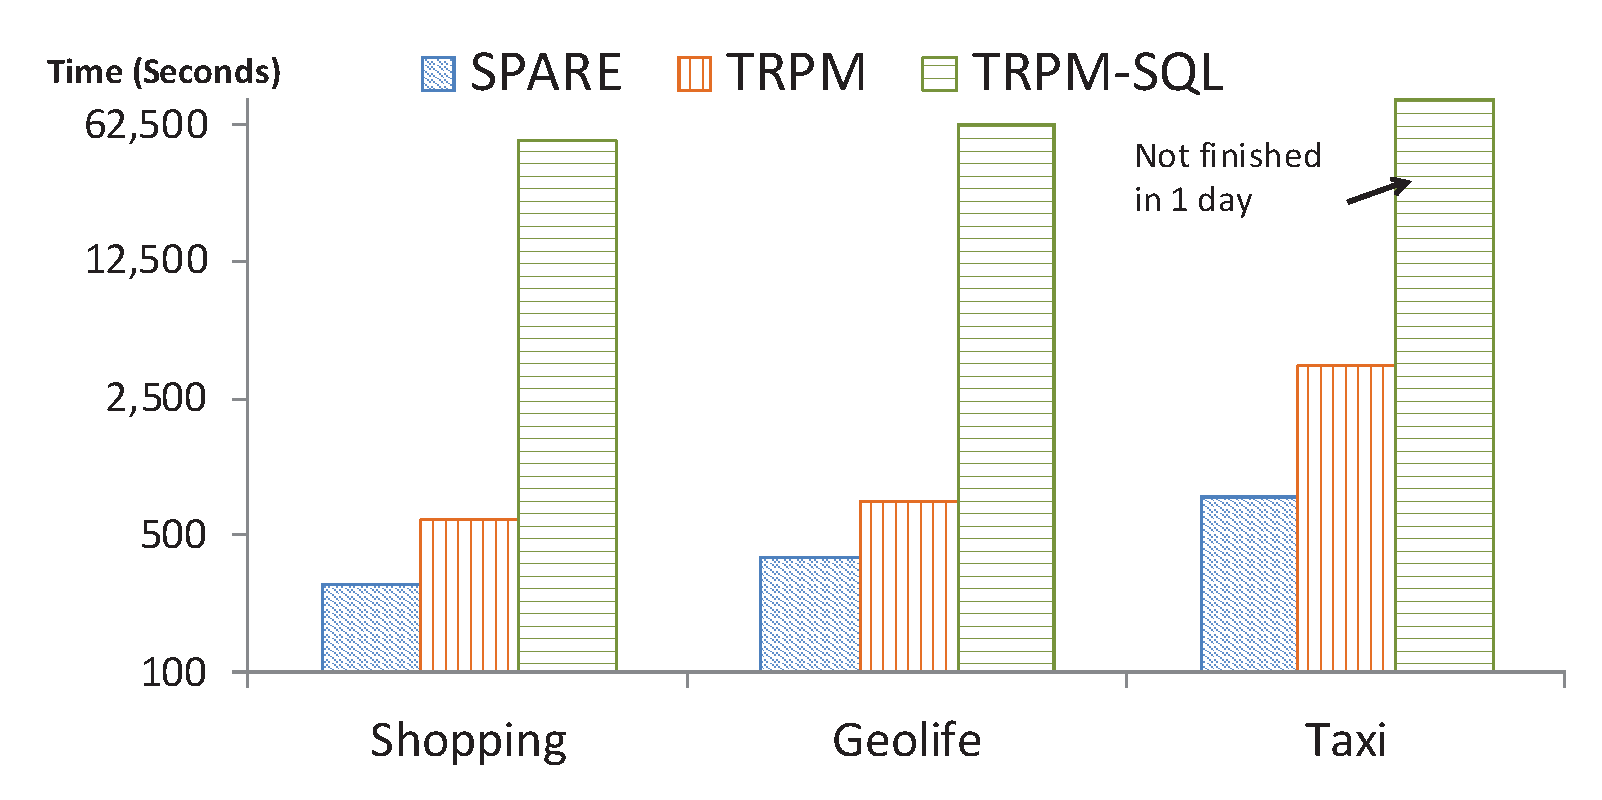
\includegraphics[width=0.4\textwidth]{spark-sql-comp.eps}
\caption{Performance comparison with SPARE, TRPM-MR and TRPM-SQL}
\end{figure}

The figure shows that TRPM-SQL is more than 120 times slower than TRPM-MR and 
takes more than 1 day in the Taxi dataset. With further investigations on the query execution
plan, 
we found that as the TRPM-SQL window query does not have a ``partition by'' clause, the Catalyst
optimizer treats the entire dataset as a SINGLE partition. This 
large partition is sent to only ONE executor to process. Such a plan
surrenders all the parallel benefits of the Spark system. Therefore, in our revised paper, we
still use the original Map-Reduce based TRPM for the performance comparisons.
% 
%
%
%To our surprise, such a window function based implementation DOES NOT perform well. The reason is that
%in TRPM, there is NO ``partition by'' clause. In such a case, Spark-SQL catalyst optimizer will treat
%the entire dataset as ONE big partition and run the UDAF for every window frame in ONE executor. We observe
%this from the physical query plan generated by Spark-Catalyst optimizer. This is no-doubt very inefficient,
%which results in a over 150 times slower than our current TRPM implementation. This performance
%of SPARE, TRPM-MR, TRPM-SQL for the three datasets are presented as follows:


%Though it is not supported in Spark 2.0.0, processing each window frame in parallel 
%can be easily implemented using simple Map-Reduce framework. However, such an processing logic
%then becomes identical to our TRPM algorithm.

\eat{
First, we think it is difficult to directly apply the window-based function with existing Spark API in the current version of Spark-SQL. This is because in both the stable Spark 1.5.2 and the newly released Spark 1.6.2, \textit{user defined aggregate function} (UDAF) on window operator is not supported\footnote{Window function improvements: \url{https://issues.apache.org/jira/browse/SPARK-7712}}. 
Without UDAF, we cannot apply our Line Sweep algorithm on the window functions. %Nevertheless, we believe UDAF may be supported in the future release and in that case,

%
Second, the performance boost on TRPM from Spark-SQL may be limited. From our investigations on the current source code of Spark-SQL\footnote{Available in Github: \url{https://github.com/apache/spark/blob/master/sql}}, its implementation
on window functions does not leverage the properties of the sliding window and the aggregate functions\footnote{Performance improvements on running window frame: \url{https://issues.apache.org/jira/browse/SPARK-8638}}. Instead, it treats each window frame independently and processes them separately. The processing logic then becomes identical to our TPRM algorithm.}
%We agree that leveraging more advanced Spark features
%could further improve the performance of our solutions. 
%We do not heavily leverage these features because 
%we wish to focus on designing parallel GCMP mining algorithms.
%%to provide a general parallel framework which does not tie to Spark.
%Nevertheless, we are in progress in developing
%a better open-sourced version with Spark-tailored optimization. 
%In the revision, we try to add a DataFrame based TRPM solution 
%which aims to leverage the window functions from Spark-SQL.
%However, to the best of our efforts, we could not achieve this goal in a short time. 
%The major challenge is that current Spark do not support User Defined Aggregate Function (UDAF)
%in window functions~\footnote{JIRA Spakr-8641: Native Spark Window Functions \url{https://issues.apache.org/jira/browse/SPARK-8641}}. Without UDAF, implementing
%our Line sweep algorithm (Algorithm 1) using Spark primitives (e.g., sum, avg, rank and nth-tile)
%is nontrivial. Nonetheless, we expect less performance
%boost from TRPM even with the UDAF support. This is because the Line sweep algorithm is not
%properly reducible, where Spark system would fail to leverage the partial aggregates
%across multiple windows. As a result, it would be equivalent to our current TRPM
%solution where windows are processed independently in parallel.
%TRPM although can be modeled using window functions over data frame, the aggregates
%it uses (i.e., the Line Sweeping method in Algorithm 1) cannot be simply represented
%by Spark primitives (e.g., sum, avg, rank, nth-tile). We then resort to
%the Spark User Defined Aggregate Function (UDAF). However, in Spark 1.5.2, the UDAF
%does not support window function syntax. Even in the latest Spark 1.6.0 (released 
%last month), UDAF does not fit with window function. We confirm these information
%with Spark development team~\footnote{In Spark JIRA tickets, fully supporting UDAF is still under development}.
%
%Nevertheless, since our Algorithm 1 is not reducible, even with UDAF, TRPM could
%not boost too much 
%
%we expect
%even with UDAF support TRPM would not boost too much.  Spark system is 
%%hard to leverage the partial aggregates acrocess
%
%we can analytically expect even using UDAF, TRPM would
%not boost too much. This is because our Algorithm 1 is not reducible. That
%is we cannot merge or share partial aggregates across different windows. In summary,
%We wish to convince the reviewer that current TRPM implementation is reasonable. 


\textbf{3.2:} \emph{Most implementations
on Hadoop and Spark are very sensitive to data partitions, i.e. prone to data
skewing issues. It seems that the (starpartition)
implementation does not take
this into account, and only use the default partitioning. It would be very helpful
to have a discussion on this topic.}

\textbf{Response:} In this paper, we actually have studied the skewness issue. In Section 5.3, we propose a best-fit strategy for SPARE to achieve a better workload balance among the reducers because star partitioning may result in partitions with a different number of nodes. In the experimental study in Section 6.2.2, we compare the SPARE algorithm with SPARE-RD and the latter only adopts the default random partition strategy. We present the summary of the execution time for each method on the longest job and standard deviation of all jobs in Table 9. The results show that SPARE demonstrates better load balance (lower deviation)
than SPARE-RD, which verifies the effectiveness of the best-fit strategy. 
%Further, TRPM generally keeps a low deviation. This is because that TRPM always adopts the equal-size (i.e. $\eta$) partition. Nevertheless, both the longest and shortest jobs in TRPM are higher than SPARE based solutions.


%We revise Section 6.2.2 by comparing TRPM, SPARE with random 
%task allocation and SPARE with best-fit task allocation (Section 5.3). We present
%the summary of the execution time for each method on longest job, shortest job and standard
%deviation of all jobs in Table 9. As the table show, SPARE has a better load balance (low deviation)
%than SPARE-RD which indicates the effectiveness of the best-fit strategy. Further, TRPM
%generally keeps a low deviation. This is because that TRPM always adopts the equal-size (i.e. $\eta$) partition.
%Nevertheless, both the longest and shortest jobs in TRPM are higher than SPARE based solutions.


\textbf{3.3:} \emph{In particular, it would be great to provide the
difference in the number of partitions/splits, the amount of processing and
memory usage (i.e., vcore and memory seconds) between TRPM and SPARE}

\textbf{Response:} In our implementation, we take a fixed 486 partitions (Section 6)
for each RDD. The partition number is determined according to
the parallel tuning guide by Cloudera\footnote{Spark Performance Tuning \url{http://blog.cloudera.com/blog/2015/03/how-to-tune-your-apache-spark-jobs-part-1/}}: there are  $3\times 54=162$ cores and each core is able to processes 3 partitions\footnote{This number may be different for other CPU models, and can be determined empirically.}
by multithreading.

Next, we add Table 7 (Section 6.1) to compare the resource usage between SPARE and TRPM in terms of Vcore-seconds, Memory and Running Time. The results show that both SPARE and TRPM are resource efficient. In particular, the RDDs for both SPARE and TRPM only take less than 20\% of the available memory. This infers that SPARE and TRPM can handle
even larger trajectory databases with our current cluster resources.



\textbf{3.4:} \emph{A plot that breaks down the performance gain by each method would
be greatly appreciated by the readers.}

\textbf{Response:} Thanks for the advice. In the revised version, we add an analysis of
the breakdown cost in Figure 8. The SPARE and TRPM algorithms have similar workflow: partitioning (Star partition v.s. $\eta$-replicate partition) in the map-shuffle phase, and  mining (Apriori Enumeration v.s. Line Sweep) in the reduce phase. %In our experiment, we treat the execution time for each phase as the cost of the corresponding methods.
As shown in Figure 8,
both star partitioning and apriori enumeration contribute to 
the final performance gain of SPARE. More specifically, in the map-shuffle phase,
SPARE saves 56\%-73\% in time as compared to TRPM. This indicates that 
fewer data are transformed and shuffled in the star partitioning.
In the reduce phase, SPARE saves 46\%-81\% time as compared to TRPM. This confirms 
the efficiency of our Apriori enumerator.

% with various optimization (e.g., sequence simplification, anti-monotonicity and forward closure checking).


\textbf{3.5} \emph{Some choices of words may need to be reconsidered: for example, ``a bunch
of" might not be appropriate in a technical paper.}

\textbf{Response:} We have changed these unprofessional terms.



\textbf{3.6} \emph{References to star partitioning and apriori pruning are missing. Though these
are well known, they need to  be clearly cited.}

\textbf{Response:} We have added the corresponding references in Section 5.1 and Section 5.2 when describing our algorithms.

\textbf{3.7} \emph{In ``In contrast, when utilizing the multicore
environment, SPAREP achieves 7 times speedup and SPARES achieves 10 times speedup.", was ``multicore"
referring to the use of all 16 cores in one of your node? The specification of the machine was not clear.}

\textbf{Response:} We used all cores in the single node (i.e., 4 executors each with 3 cores) to conduct the experiment. We have revised the description in Section 6.2.3.



\textbf{3.8} \emph{The computation of "eta" was slightly different than that in the paper}

\textbf{Response:} Thanks for pointing this out. We have updated the GitHub repository to rectify the typo in the equation.



\section{Response to Reviewer 1}

\emph{The main con that I've spotted is the fact that the algorithm might have been
more nicely framed also within the Spark environment by taking advantage of
the various possibilities offered by it (e.g. caching of RDDs)}

\response{We agree that utilizing advanced Spark features would 
improve our solutions. In this work, we do not include 
these optimization in-depth because we set out focus 
on solving the challenges in parallelizing the 
GCMP mining algorithms.
We are also in progress of open-sourcing a Spark-tailored
version of SPARE.
} 


\section{Response to Review 2}

\textbf{2.1} \emph{The GCMP generalization is not particularly novel. Putting a maximum gap size
on consecutive segments is well-known
in sequence mining published more than
10 years ago.}

\textbf{Response:}
We admit that the gap parameter is also used in
mining Gap-restricted Sequential Patterns (GSP). 
However, the novelty of this paper lies
on the one-stop solution of mining co-movement patterns.
In modeling, we provide the generalize co-movement pattern to
alleviate the troubles
is not merely on introducing the gap-constraint.
Instead, we provide a one-stop solution for mining co-movement patterns. With
our 

However, the novelty
of this paper is not merely on introducing the gap-constraint to the generalized
co-movement pattern. 
Instead, we provide a one-stop solution (both in modeling and in technical)
for mining various co-movement patterns with flexible constraints.
 

This solution not only alleviate the cumbersome for designing each
individual patterns, but also 

 With
these constraints, users are able to define a more accurate pattern
which are free from the anomalies (e.g., loss-connection anomaly in Figure 2).

Besides, the essence of GSP and GCMP are different. The goal of GSP 
is to find the sequences which conform to the gap constraint and occur frequently.
When counting the occurrence of a sequence in GSP, the object
which a sequence belongs to does not matter. Therefore, 
in a GSP result, the involved objects may be neither
 distinct nor close.
In contrast, GCMP imposes requirements on both the spatial closeness 
of objects and the number of distinct objects.
Due to the unawareness of objects, techniques that are used in GSP 
cannot be directly applied on GCMP. We summarize this difference
in Section 2.5.


\emph{In fact, I have doubts about formulating the GCMP patterns as proposed. Are
we really interested in all sets of movements beyond a cardinality of size $M$? 
Take the Taxi dataset as an example. Let say that there are lots of taxis going
from the airport to downtown. Let say that there are 1000 such taxis. For a
given $M$, are we interested in ${1000 \choose M}$ answers? 
So this speaks to the problem of picking $M$. If $M$ is 500, what is ${1000 \choose M}$? In fact, even if the
system gives the single answer of ${1000\choose 1000}$,
I am not sure I am
interested in this pattern as I already know that there are many taxis going from
the airport to downtown. What I think I am really interested in are GCMP that
are ``anomalous'', which is much harder to define.}

\response{We appreciate the reviewer's concerns on the 
size of the output. 
In fact, both TRPM and SPARE
have considered compressing the output by only discovering 
the patterns with larger object set. 
Particularly,  in the Line Sweeping Mining (Algorithm 1) of TRPM, whenever
a pattern $c$ becomes valid, it is directly outputted (Lines 14-16). This
prohibits outputting $c$'s subset. Similarly, in the Apriori Enumerator (Algorithm 3)
of SPARE, a pattern $c$ is outputted if none of its supersets could become a valid pattern (Line 12-14).
This ensures the output $c$ is not a subset of some pattern.
These mechanisms effectively condense the output by subsuming smaller
patterns using their supersets.
% Nevertheless, these mechanisms are able to preserve ALL valid patterns.
Linking to the Taxi example, if the ground truth contains 1000 taxis travel
together, then both TRPM and SPARE tend to output the single pattern.
In addition, real detection of ``anomalous'' co-moment pattern needs to 
impose stringent constraints via $M,K,L,G$. This would further reduces 
the size of the output.
%On the other hand, in reality, if users wish to detect ``anomalous'' patterns,
%the parameters $M,K,L,G$ will be set to be very stringent. This reduces
%the size of potential outputs. For example, when detecting the Taxi's movements
%without ground truth of 1000 taxis, an input could be $M = 100$, $K=50$ min, $L=30$ min,
%$G = 2$ min. Then, there would be very less patterns satisfying these constraints.
% and the meaningfulness of the output. 
%In terms of the output size, 
%we certainly do not need to output every pattern.
%In fact, both TRPM and SPARE algorithms tend to only output
%the patterns with larger object size. That is to say, for
%the Taxi example, the pattern containing all the 1000 taxis will
%be outputted. To see this, in Algorithm 1, TRPM effectively 
%starts with a temporally invalid pattern and continue
%to shrink its object set until it is temporally valid. Then, the result
%is the ``largest'' valid pattern for these object. Similarly,
%in Algorithm 3, SPARE effectively starts with a temporally valid
%pattern with small object set. Then SPARE continues to grow
%the object set until its temporal dimension is about to be non-decomposable (Definition 5).
%Therefore both TRPM and SPARE tends to find the ``largest'' valid
%patterns.
%
%In terms of the meaningfulness, we believe that all patterns that conformed
%to the parameters need to be outputted. 
%This is because the parameters
%
%
%We see two questions derived from this concern. First, do we need
%to output all ${1000 \choose M}$ patterns if $1000$ taxis form a true GCMP
%pattern? Our answer to this question is no. Therefore, the nature of both
%of our TRPM and SPARE algorithms tend to only output the patterns containing 
%larger sets of objects. To see this, in Algorithm 1, TRPM starts with an temporal invalid
%pattern and continues to shrink its object set while growing its temporal dimension.
%TRPM stops as soon as the object become valid. In an inverse way, in Algorithm 3, 
%SPARE starts with a pattern with small objects and continues to grow its object set
%while reducing its temporal dimension. SPARE stops as soon as the pattern is about
%to be temporally invalid. Therefore, both TRPM and SPARE would prefer to output
%larger pattern.
%
%
%%
%%We agree with the reviewer that if no other parameters are given, the maximum number
%%of patterns discovered could be as large as ${ \mathbb{O} \choose M}$, which may
%%be less interesting to users.
%However, such a case rarely occurs due to two reasons. First,
%in real trajectory mining, parameter $M$
%is associated with temporal parameters $K,L,G$ and they jointly prune many false
%patterns. Second, the nature of our solutions prefer 
%a larger pattern when possible~\footnote{TRPM shrinks an invalid larger pattern until it is valid. SPARE grows a valid smaller pattern until it is about to be invalid. Therefore both algorithms tend to find larger patterns.}.
%For example, if $(o_1,o_2,o_3)$ is 
%a pattern and $M = 2$, 
%then both TRPM and SPARE only output $(o_1,o_2,o_3)$ but not
%any of its subsets. This effectively compresses smaller patterns.
%
%In addition, when the temporal parameters $K,L,G$ are given,
%a larger $M$ actually decreases the number of resulted patterns. 
%This is because there are less patterns having more than $M$ objects. 
%As shown in Figures 7 (a)(g)(m), a larger $M$ actually reduces the running time of both TRPM and SPARE.
}

\emph{Regarding the second weak points, one line of related work is the superimposition
of constraints on spatiotemporal mining. An example is a road network. In other words, given a road network, the network imposes constraints on GCMP.}

\response{We understand that spatiotemporal mining with domain-constraints
looks similar to GCMP.
However, those techniques often heavily utilize the domain knowledge (such as
directions in road networks) which are nontrivial to be generalized.
Differently, since our GCMP model and technical solutions
do not leverage the domain knowledge, we can support
pattern discovery in broader scenarios such as user check-in histories in social networks, visitor movements in a building and 
passenger flows in a city. We also add the discussion in Section 2.3.
}
\section{Responses to Reviewer 3}
\emph{Though the implementation references Spark as the implementation
platform (as it also reflects in github repo provided), the algorithm design is
mostly limited to MapReduce, aka only Hadoop, which is a very small subset of
Spark. This may have a negative impact on the baseline implementation.
Particularly, recent releases of Spark have introduced window functions that can
be applied directly in the sliding window scenario here. Certainly, the algorithm
has to be redesigned to use DataFrame (and/or Spark SQL) interface, it has
been noted that this is a very efficient way to execute window functions in
Spark}

\response{
We thank the reviewer for suggesting a better way of implementing 
the baseline algorithm (i.e., TRPM). However, this could
hardly be done after our investigations. The major reason is
that current version of Spark SQL (i.e., 1.6.2 released in June)
does not support the User Defined Aggregate Function (UDAF) on window
function~\footnote{JIRA Spakr-8641: Native Spark Window Functions \url{https://issues.apache.org/jira/browse/SPARK-8641}}. Without UDAF, implementing
our Line sweep algorithm (Algorithm 1) using Spark SQL 
primitive aggregates (e.g., sum, avg, rank and nth-tile)
is beyond our abilities.

Further, we believe the performance boost on TRPM from Spark SQL
is very limited. The reason is that our 
Line Sweeping Mining algorithm (Algorithm 1) is not a 
properly reducible function. That is, the result of a 
smaller window could not be used to compute the result of a larger
window. In such a case, Spark SQL has to process each
window independently in parallel, which is equivalent to our TRPM implementation.
%We agree that leveraging more advanced Spark features
%could further improve the performance of our solutions. 
%We do not heavily leverage these features because 
%we wish to focus on designing parallel GCMP mining algorithms.
%%to provide a general parallel framework which does not tie to Spark.
%Nevertheless, we are in progress in developing
%a better open-sourced version with Spark-tailored optimization. 
%In the revision, we try to add a DataFrame based TRPM solution 
%which aims to leverage the window functions from Spark-SQL.
%However, to the best of our efforts, we could not achieve this goal in a short time. 
%The major challenge is that current Spark do not support User Defined Aggregate Function (UDAF)
%in window functions~\footnote{JIRA Spakr-8641: Native Spark Window Functions \url{https://issues.apache.org/jira/browse/SPARK-8641}}. Without UDAF, implementing
%our Line sweep algorithm (Algorithm 1) using Spark primitives (e.g., sum, avg, rank and nth-tile)
%is nontrivial. Nonetheless, we expect less performance
%boost from TRPM even with the UDAF support. This is because the Line sweep algorithm is not
%properly reducible, where Spark system would fail to leverage the partial aggregates
%across multiple windows. As a result, it would be equivalent to our current TRPM
%solution where windows are processed independently in parallel.
%TRPM although can be modeled using window functions over data frame, the aggregates
%it uses (i.e., the Line Sweeping method in Algorithm 1) cannot be simply represented
%by Spark primitives (e.g., sum, avg, rank, nth-tile). We then resort to
%the Spark User Defined Aggregate Function (UDAF). However, in Spark 1.5.2, the UDAF
%does not support window function syntax. Even in the latest Spark 1.6.0 (released 
%last month), UDAF does not fit with window function. We confirm these information
%with Spark development team~\footnote{In Spark JIRA tickets, fully supporting UDAF is still under development}.
%
%Nevertheless, since our Algorithm 1 is not reducible, even with UDAF, TRPM could
%not boost too much 
%
%we expect
%even with UDAF support TRPM would not boost too much.  Spark system is 
%%hard to leverage the partial aggregates acrocess
%
%we can analytically expect even using UDAF, TRPM would
%not boost too much. This is because our Algorithm 1 is not reducible. That
%is we cannot merge or share partial aggregates across different windows. In summary,
%We wish to convince the reviewer that current TRPM implementation is reasonable. 
}

\emph{In particular, it would be great to provide the
difference in the number of partitions/splits, the amount of processing and
memory usage (i.e., vcore and memory seconds) between TRPM and SPARE}

\response{We add Table 7 to include vcore-seconds 
and RDD memory usage for both TRPM and SPARE. We also add a clear description on partitions in Section 6.
}


\emph{A plot that breaks down the performance gain by each method would
be greatly appreciated by the readers.}

\response{We complement Figure 8 with the breakdown cost of TRPM. This
comparison showcases the benefits of both Star Partition (in mapshufle phase)
and Apriori Enumeration (in reduce phase) of SPARE.
}

\emph{Some choices of words may need to be reconsidered: for example, "a bunch
of" might not be appropriate in a technical paper.}

\response{We thank the reviewer for the correction. We have changed many unprofessional terms.
}


\emph{References to star partitioning and apriori pruning are missing. Though these
are well known, they need to clearly cited. At least the following reference is
missing:}

\response{We add the corresponding references in Section 5.1 and Section 5.2.}

\emph{In "In contrast, when utilizing the multicore
environment, SPAREP achieves 7 times speedup and SPARES achieves 10 times speedup.", was "multicore"
referring to the use of all 16 cores in one of your node? The specification of the machine was not clear.}

\response{ We use all cores in a single node to conduct the experiments. We revise the description in Section 6.2.3.
} 


\emph{The computation of "eta" was slightly different than that in the paper}

\response{
We have updated the GitHub repository to rectify the typo in the equation.}
\section{Response to Meta Reviewer}

\textbf{M.1} \emph{Novelty: The GCMP generalization is not particularly novel. Please elaborate on the novelty of the work.}

\textbf{Response:} In addition to the points in the response of comments 2.1, another novelty of our work lies in the 
techniques. 
Although the idea of star partition and apriori enumeration are well-known, 
linking them together to solve the problem in trajectory domain has not been attempted before.
Besides, we input heavy details on these algorithms (e.g., theoretical bounds of partition and
anti-monotonicity) which have not been previously proposed.


\textbf{M.2} \emph{Parameter setting: Are we really interested in all sets of movements beyond a cardinality of size M? Please elaborate
on the motivation.}

\textbf{Response:} Addressed in the response for comments 2.2. 

\textbf{M.3} \emph{Spark implementation: the paper references Spark as the implementation platform but the algorithm is limited to MapReduce. Spark has capabilities beyond MapReduce such as window functions. Please provide an implementation that uses the relevant features of Spark, or a convincing discussion of how these features can be useful and why they were not used.}

\textbf{Response:} Addressed in the response for comments 1.1 and 3.1.

\textbf{M.4} \emph{More details in the performance evaluation: Please provide more details about data partitioning and the effect of skew. Also provide details about how star partitioning and a priori pruning contribute to performance. Please provide references to these two methods.}

\textbf{Response:} Addressed in the response for comments 3.2, 3.3, 3.4 and 3.6.




%%%%%%%%%%%%%%%%%%%%%%%%%%%%%%%%%%%%%%%%%%%%%%%%%%%%%%%%%%%%%%%%%%%%%%%%%
%%%%%%%%%%%%%%%%%%%%%%%%%%%%%%%%%%%%%%%%%%%%%%%%%%%%%%%%%%%%%%%%%%%%%%%%%
%%%%%%%%%%%%%%%%%%%%%%%%%%%%%%%%%%%%%%%%%%%%%%%%%%%%%%%%%%%%%%%%%%%%%%%%%



\section{Response to Meta Reviewer}

\textbf{M.1} \emph{Novelty: The GCMP generalization is not particularly novel. Please elaborate on the novelty of the work.}

\textbf{Response:} The novelty of the paper includes:
\begin{itemize}
\item We are the first to incorporate the parameter of maximum gap in the co-movement pattern definition.

\item We are the first to deploy a distributed solution framework on Spark to solve the generalized pattern mining problem.

\item There are also several novel ideas in our SPARE algorithm. For example, we devise a novel Star Partitioning to achieve better workload balance. In order to apply Apriori algorithm to overcome the exponential enumeration problem, we also devise novel concepts of sequence simplification to find a new type of monotonicity which can significantly reduce the number of candidates. 
\end{itemize}

\eat{

In addition to our response to comments 2.1, another novelty of our work lies in the 
techniques. 
Although the idea of star partition and apriori enumeration are well-known, 
linking them together to solve the problem in trajectory domain has not been attempted before.
Besides, we input heavy details on these algorithms (e.g., theoretical bounds of partition and
anti-monotonicity) which have not been previously proposed yet.
}


\textbf{M.2} \emph{Parameter setting: Are we really interested in all sets of movements beyond a cardinality of size M? Please elaborate
on the motivation.}

\textbf{Response:} We address this issue in Comment 2.2. 

\textbf{M.3} \emph{Spark implementation: the paper references Spark as the implementation platform but the algorithm is limited to MapReduce. Spark has capabilities beyond MapReduce such as window functions. Please provide an implementation that uses the relevant features of Spark, or a convincing discussion of how these features can be useful and why they were not used.}

\textbf{Response:} We address this issue in Comments 1.1 and 3.1.

\textbf{M.4} \emph{More details in the performance evaluation: Please provide more details about data partitioning and the effect of skew. Also provide details about how star partitioning and a priori pruning contribute to performance. Please provide references to these two methods.}

\textbf{Response:} We address these issues in 3.2, 3.3, 3.4 and 3.6.

\end{document}